%!TEX root = /Users/dbreuer/Documents/Work/_FH/_Master/master_thesis/Main/Master Thesis.tex

\chapter{COSIMA - Eine dienstorientierten Multimediaarchitektur} % (fold)
\label{cha:eine_dienstorientierten_multimediaarchitektur}

  Im Abschnitt~\ref{sec:motivation} wurde bereits kurz darauf eingegangen, dass die vorliegenden Arbeit vor dem Hintergrund des COSIMA-Projekts entstanden ist. In diesem Kapitel soll dieses Projekt so weit vorgestellt werden, dass für den weiteren Verlauf der Arbeit ein grundlegendes Verständnis über die Ziele, Alleinstellungsmerkmale und Herausforderungen existiert.
  
\section{Motivation} % (fold)
\label{sec:motivation_cosima}

  Das COSIMA-Projekt ist aus dem Wahlpflichtfach Modellierung in audio-visuellen Medien (MIAV\abk{MIAV}{Modellierung in audio-visuellen Medien}) an der Fachhochschule Köln im Masterstudiengang der Medieninformatik hervorgegangen. Im Rahmen einer Projektarbeit wurde das die Projektidee weiter ausgearbeitet und konzipieren. Die Ergebnisse dieser Arbeit wurden als Institutsbericht an Fachhochschule Köln bereitsgestellt und sind dort im Detail einsehbar~\citep{bericht}.
  
  Das folgende Kapitel wird daher nur auf die wesentliche Punkte des COSIMA-Projekts eingehen und ihre Relevanz für diese Arbeit herausstellen. Die ursprüngliche Idee hinter COSIMA war es ein Framework zu entwickeln, dass die Entwicklung von Multimediaanwendungen vereinfacht. Im Gegensatz zu anderen Medienframeworks, wie etwa dem \emph{Java Media Framework} (JMF\abk{JMF}{Java Media Framework}), wurde bei dem COSIMA-Projekt ein ganzheitlicher Ansatz verfolgt.
  
  Im Institutsbericht wird darauf hingewiesen, "`dass die Entwicklung von Multimediaanwendungen derzeit verhältnismässig aufwendig ist"'~\citep[S. 2]{bericht}. Eine Ursache dieser Problematik, liegt nach Aussage der Autoren darin begründet, dass sich die zur Zeit verfügbaren Rahmenwerke im Bereich der Multimediaverarbeitung auf einen sehr engen Einsatzbereich beschränken. Neben JMF sind hier zusätzlich noch \emph{QuickTime}\footnote{\url{http://www.apple.com/quicktime/}} und \emph{ImageJ}\footnote{\url{http://rsbweb.nih.gov/ij/}} zu nennen. Andere Aspekte von Multimediaanwendungen, wie etwa die Integration von Metadaten, müssten von dem Anwendungsentwickler erst manuell mit diesen Rahmenwerken integriert werden. "`Ein Meta-Framework, welches die bestehenden Ansätze verbinden und integrieren könnte, würde die Wiederverwendbarkeit und generelle Entwicklungsarbeit positiv beeinflussen, beziehungsweise vereinfachen"'~\citep[S. 3]{bericht}, wird von den Autoren des Berichts daher als Bestreben hinter dem COSIMA-Projekt angeführt.
  
  Neben der Notwendigkeit ein \emph{Meta-Framework}\footnote{Das ursprüngliche Ziel war tatsächlich ein Framework zu schaffen. Erst während der Validierung im Rahmen dieser Arbeit ist zu Tage gekommen, dass es sich mehr um eine Architektur handelt und weniger um ein Framework. Im weiteren Verlauf wird darauf jedoch noch genauer eingegangen.} zu schaffen, führen die Autoren als weiteren Beweggrund das Fehlen einer Architektur für Multimediaanwendungen an. Innerhalb dieser Architektur könnten sich Anwendungsentwickler wesentlicher effektiver bewegen und müssten nicht erst eine eigene Architektur von Grund auf entwerfen.
  
  Da sich mit den meisten bestehenden Multimedia-Rahmenwerke keine verteilten Anwendungen realisieren lassen, lag auch dieser Aspekt von Beginn an im Fokus der Konzeptionierung. Als Grundlage eine geeignete Architektur zu konzipieren, die es ermöglicht, verteilte Anwendungen zu realisieren, diente das Konzept der \emph{Service-oriented Architecture} (SOA\abk{SOA}{Service-oriented Architecture}) oder \emph{Dienst-orientierten Architektur}.
  
  Die hier aufgeführten Punkte haben initial die Entwicklung eines Rahmenwerkes motiviert, dass später im COSIMA-Projekt aufgehen sollte. Die im Verlauf der Projektarbeit entwickelten Ziele von COSIMA sind im nächsten Abschnitt zusammen gefasst.

% section motivation_cosima (end)
  
\section{Ziele} % (fold)
\label{sec:ziele_cosima}

  Das \emph{Mission Statement} des COSIMA-Projekts fasst bereits alle Ziele des Projekts in einer Kernaussage zusammen:

  \begin{quote}
    \emph{``MIAV ist ein integratives, komponentenbasiertes Meta-Framework mit gezielter Ausrichtung auf Multimediaverarbeitung. Es vereinfacht die Entwicklung von verteilten Multimedia-Applikationen durch eine flexible, dienst-orientierte Architektur. Die Wiederverwendbarkeit von Komponenten und bestehenden Frameworks wird dadurch begünstigt.''} (aus~\citep[S. 2]{bericht})\footnote{Die Bezeichnung "`COSIMA"' hat das Projekt erst nach Fertigstellung des Berichts erhalten, daher findest sich hier noch die zuvor verwandte provisorische Bezeichnung \emph{MIAV-Framework}.}
  \end{quote}

  Neben den zentralen Aspekten \emph{dienst-orientierte Architektur}, \emph{Integration} und \emph{Meta-Framework}, die im Abschnitt zuvor bereits dargestellt wurden, nennen die Autoren hier zusätzlich noch die Aspekte der \emph{komponentenbasierten Architektur}, \emph{Wiederverwendbarkeit} und natürlich der \emph{Medienverarbeitung}.
  
  Neben den hier genannten Zielen, die das COSIMA-Projekt zu erreichen versucht, zeichnet sich das Projekt durch seine spezifischen Charakteristika in Bezug auf andere Multimedia-Rahmenwerke aus. Diese Alleinstellungsmerkmale werden im nächsten Abschnitt genauer betrachtet.

  % - Welche Ziele verfolgt das COSIMA-Projekt?
  % - Warum handelt es sich um eine Architektur und nicht um ein Framework!!!! (Im Bericht noch anders, irgendwie muss das hier verwurstet werden!)
  % - Weiterentwicklung der Definition seit dem Bericht

% section ziele_cosima (end)

\section{Alleinstellungsmerkmale} % (fold)
\label{sec:alleinstellungsmerkmale}

  Aus den in Abschnitt~\ref{sec:ziele_cosima} dargestellten Zielen des COSIMA-Projekts lassen sich die folgenden Merkmale extrahieren, die COSIMA im Bereich der Multimedia-Rahmenwerke und -Anwendungen einmalig machen~\citep[S. 3f]{bericht}:
  
  \begin{description}
    \item[Verteiltheit] COSIMA ist konzipiert als ein verteiltes System.
    \item[Dienstorientierung] Angelehnt an die \emph{Service-Oriented Architecture} (SOA), sind die Bausteine in COSIMA als Dienste modelliert.
    \item[Integration] Bestehende Frameworks können in Form von Diensten angeboten und so ihre Funktionalität eingebunden werden.
    \item[Erweiterbarkeit] Die Dienstorientierung erlaubt die Einbindung eigener Komponenten.
    \item[Skalierbarkeit] In einer verteilten, dezentralisierten Umgebung können einzelne Funktionalitäten als Dienste völlig unabhängig voneinander betrieben werden. Die Folge ist die vollständige Flexibilität in Bezug auf die Skalierbarkeit des gesamten Systems~\citep[S. 294]{web_services_principles_and_technology}.
    \item[Medienobjekt-Modellierung] Modellierung von Medien in ganzheitlicher Betrachtungsweise von Rohdaten und Metadaten in einem Objekt.
    \item[Meta-Ebene] COSIMA fokussiert nicht auf Datensicht oder Metadatensicht sondern abstrahiert auf höhere Ebene.
    \item[Medienverarbeitung] Ganzheitliche Sicht auf Medienverarbeitung: Produktion, Verarbeitung, Transformation, Anreicherung, Wiedergabe, Ausgabe von Daten und Metadaten.
    \item[Architektur] COSIMA stellt eine Architektur für Multimediaanwendungen.
  \end{description}
  
  Basierend auf den vorgestellten Zielen und Alleinstellungsmerkmalen wurde die Architektur entworfen, die in dieser Arbeit validiert und prototypisch realisiert wurde. Im Folgenden Abschnitt wird diese Architektur im Detail vorgestellt werden.

% section alleinstellungsmerkmale (end)

\section{Architektur} % (fold)
\label{sec:architektur}

  Die Architektur des COSIMA-Projekts ist iterativ in einem dedizierten Vorgehen\footnote{Dieses Vorgehen wird detailliert im Institutsbericht vorgestellt. Eine Erläuterung in diesem Rahmen ist nicht angemessen und wird daher ausgelassen.} bis zu dem Punkt entwickelt worden, der als Ausgangspunkt für die Betrachtungen in dieser Arbeit dient. Bevor dieser aktuelle Stand jedoch in den folgenden Abschnitten im Detail vorgestellt wird, soll zunächst einmal der Begriff Architektur definiert und eingeordnet werden.
  
\subsection{Definition: Software Architekturen} % (fold)
\label{sub:definition_software_architekturen}

  Der Begriff der Architektur im Kontext der Softwaretechnik und -entwicklung lässt sich sehr breit fassen. Es existieren unzählige Bücher zu dem Thema und allein das Software Engineering Institute (SEI)\abk{SEI}{Software Engineering Institute} der Carnegie Mellon Universität hat online bisher über 80 Definition von Architektur zusammen getragen\footnote{\url{http://www.sei.cmu.edu/architecture/definitions.html}, zuletzt abgerufen am 03. November 2008}. Daher soll an dieser Stelle eine Einordnung des Begriffs der Software Architektur vorgestellt werden, wie er in dieser Arbeit Verwendung findet.
  
\subsubsection{Definitionen} % (fold)
\label{ssub:definitionen}

  Das IEEE definiert in ihrem Glossar zur Softwaretechnik den Begriff Architektur wie folgt:
  
  \begin{definition}[Architektur (IEEE)]\label{def:architektur_ieee}
    "`The organizational structure of a system or component. See also: component; module; subprogram; routine"'~\emph{\citep{ieee90sg}.}
  \end{definition}
  
  Diese sehr einfache Definition von Architektur weist schon auf die Eigenschaft der Strukturierung hin. Die Auswahl der folgenden Definitionen stellen die Eigenschaften von Architektur aber noch einmal klarer heraus.
  
  \begin{definition}[Architektur (Crispen)]\label{def:architektur_crispen}
    "`An architecture [\ldots] consists of (a) a partitioning strategy and (b) a coordination strategy. The partitioning strategy leads to dividing the entire system into discrete, non-overlapping parts or components. The coordination strategy leads to explicitly defined interfaces between those parts."'~\emph{\citep[S. 272]{crispen1994sm}}
  \end{definition}
  
  \begin{definition}[Architektur (Reussner et al.)]\label{def:architektur_reussner_et_al}
    "`Die Software-Architektur ist die grundlegende Organisation eines Systems, dargestellt durch dessen Komponenten, deren Beziehungen zueinander und zur Umgebung, sowie die Prinzipien, die den Entwurf und die Evolution des Systems bestimmen."'~\emph{\citep[S. 1]{handbuch_der_software_architektur}}
  \end{definition}
  
  \begin{definition}[Architektur (Bass et al.)]\label{def:architektur_bass_et_al}
    "`The software architecture of a program or computing system is the structure or structures of the system, which comprise software components, the externally visible properties of those components, and the relationship among them."'~\emph{\citep[S. 21]{software_architecture_in_practice}}
  \end{definition}
  
  Darüber hinaus ist noch die Unterscheidung von \emph{Software}- und \emph{System}-Architekturen zu treffen~\citep[S. xix]{evaluating_software_architectures}. Eine System-Architektur berücksichtigt dabei deutlich mehr Komponenten, wie etwa die Hardware und deren Umgebung auf der die Software installiert werden soll. Diese Trennung wird auch in den entsprechenden Definitionen des SEI deutlich:
  
  \begin{definition}[Software-Architektur (SEI)]\label{def:software_architektur_sei}
    "`The structure or structures of a system, which comprise the software elements, the externally visible properties of those elements, and the relationships among them."'~\emph{\citep{sei_glossary}}
  \end{definition}
  
  \begin{definition}[System-Architektur]\label{def:system_architektur}
    "`A means for describing the elements and interactions of a complete system including its hardware elements and its software elements."'~\emph{\citep{sei_glossary}}
  \end{definition}

  Bei der Architektur innerhalb des COSIMA-Projekts handelt es sich also um eine Software-Architektur, da ausschließlich die Softwarekomponenten ohne Rücksicht auf mögliche Hardware betrachtet werden. Genauer kann auch gesagt werden, dass es sich um eine Referenzarchitektur nach Reussner et al. handelt:
  
  \begin{definition}[Referenzarchitektur]\label{def:referenzarchitektur}
    "`Eine Referenzarchitektur ist eine abstrakte Software-Architektur, sie definiert Strukturen und Typen von Software-Elementen sowie deren erlaubte Interaktionen und ihre Verantwortlichkeiten speziell für einen Anwendungsbereich. Die Strukturen sind jeweils für alle Systeme innerhalb einer Domäne anwendbar."'~\emph{\citep[S. 358]{handbuch_der_software_architektur}}
  \end{definition}

% subsubsection definitionen (end)

  Die Architektur einer Software ist also die strukturelle Aufteilung der Software in einzelne, von einander unabhängige Komponenten, deren Eigenschaften und Beziehungen untereinander. Im Folgenden werden nun diese einzelnen Komponenten der COSIMA Architektur vorgestellt werden.

% subsection definition_software_architekturen (end)

\subsection{Einführung} % (fold)
\label{sub:einfuehrung}

  Bei der Konzeption und Entwicklung der Architektur sind unterschiedliche Sichten auf diese erstellt worden. Diese Sichten entsprechen denen von Starke in~\citep[S. 83]{effektive_software_architekturen} beschriebenen vier Arten von Sichten auf eine Software-Architektur: \emph{Kontextsichten}, \emph{Bausteinsichten}, \emph{Laufzeitsichten} und \emph{Verteilungssichten}.

  Für das COSIMA-Projekt wurden bisher Darstellungen aus zwei dieser Kategorien erstellt: eine der Kontextsichten und drei der Bausteinsichten. Die Kontextsichten legen laut Starke den "`Fokus auf den Zusammenhang oder das Umfeld des Systems"'~\citep[S. 87]{effektive_software_architekturen}, was auch auf die in Abbildung~\ref{fig:Kontextsicht_Architektur_COSIMA} dargestellte Kontextsicht von COSIMA zutrifft. Hier wird lediglich ein abstrakter und vor allem nicht formaler Überblick über die Architektur und beteiligte Systeme gegeben. Die Darstellungen, die sich den Bausteinsichten zuordnen lassen, sind namentlich das \emph{Komponentendiagramm}, das \emph{Kompositionsstrukturdiagramm} und der \emph{Grobentwurf} der Architektur. Diese finden sich jeweils in~\citep{bericht} und sollen an dieser Stelle nicht weiter betrachtet werden\footnote{\textbf{TODO}: Im weiteren Verlauf werden sicher Teile aus diesen Diagrammen benötigt, daher muss dann darauf referenziert werden.}. Für die weitere Vorstellung der Architektur soll an dieser Stelle die Kontextsicht genügen.

\begin{figure}[ht]
  \centering
    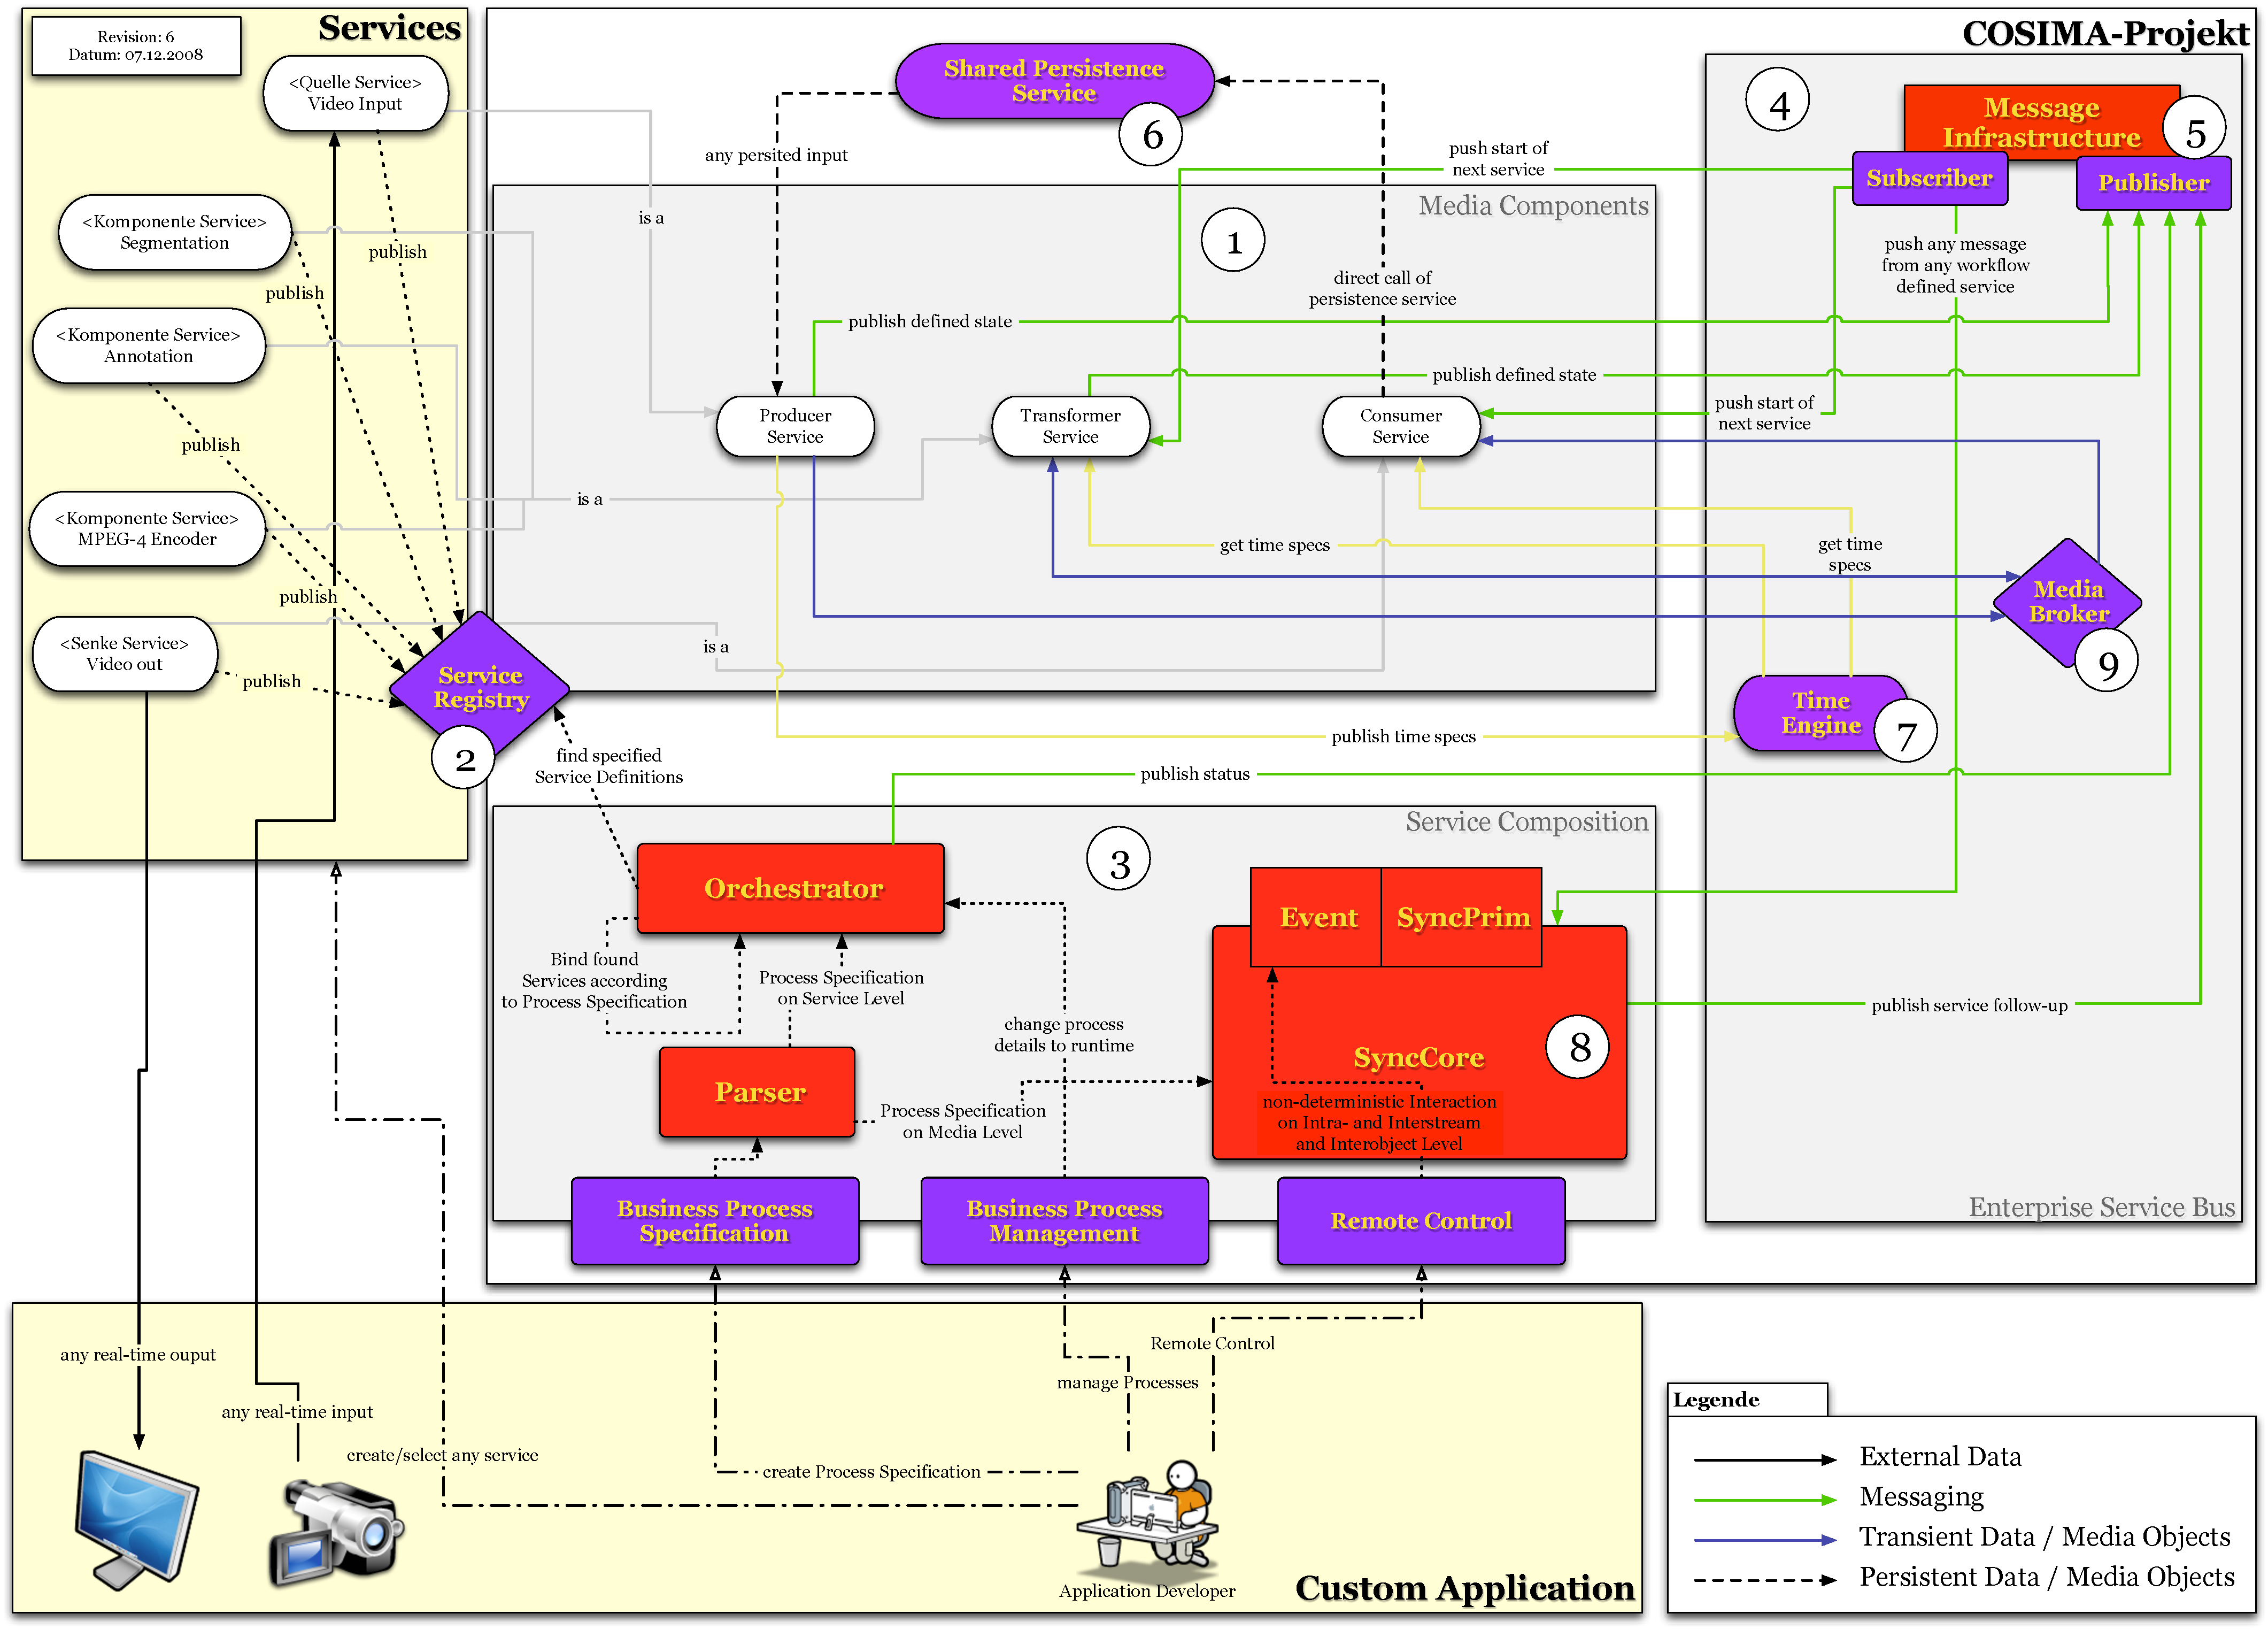
\includegraphics[width=.9\textwidth]{images/Kontextsicht_Architektur_COSIMA}
  \caption{Kontextsicht der Architektur des COSIMA-Projekts}
  \label{fig:Kontextsicht_Architektur_COSIMA}
\end{figure}

  In der späteren prototypischen Realisierung und anschließenden Validierung der Architektur sollen und können nur Fragmente der Architektur umgesetzt werden, daher ist es sehr wichtig, solche Fragmente zu wählen, die für eine Weiterentwicklung von besonderem Interesse sind. Im Folgenden werden daher die zentralen Komponenten des COSIMA-Projekts kurz vorgestellt. \emph{Später soll dann eine Auswahl getroffen werden.}

  % - Kernpunkte der Architektur herausarbeiten
  % - Diese Kernpunkte müssen in der Realisierung/Validierung entsprechend besondere Berücksichtigung finden

% subsection einfuehrung (end)

\subsection{Medienverarbeitende Komponenten} % (fold)
\label{sub:medienverarbeitende_komponenten}

  Den Kern von COSIMA machen die medienverarbeitenden Komponenten aus, die vom Anwendungsentwickler in eine entsprechende Abfolge gebracht werden und damit die später Multimediaanwendung selbst darstellen: \emph{Producer}, \emph{Transformer} und \emph{Consumer}. Dem Entwurf der Komponenten liegt das \emph{Quelle-Komponente-Senke} Prinzip zu Grunde. Die innerhalb des COSIMA-Projekts verwendete Bezeichnung ist nach~\citep{a_multimedia_component_kit,multimedia_component_frameworks} ebenso valide wie die geläufigere Bezeichnung "`Quelle-Komponente-Senke"'. Da es sich bei COSIMA jedoch um eine komponentenbasierte Architektur handelt, wodurch Benennungsschwierigkeiten aufkamen, die die Verwendung einer alternativen Begrifflichkeit begünstigten.
  
  Diese medienverarbeitenden Komponenten sind alle als Dienste ausgeprägt, um dem Anspruch der Dienstorientierung gerecht zu werden. Eine Komponente kann dabei niemals eine andere Komponente direkt aufrufen, diese Aufgabe obliegt der \emph{Service Komposition} (siehe Abschnitt~\ref{sub:service_komposition}). Jede dieser Komponenten muss sich dazu bei seiner Initiierung beim Service Repository registrieren, der in~\ref{sub:service_registry} näher beschrieben wird.
  
  Der Austausch der zu verarbeitenden Medien zwischen den einzelnen Komponenten geschieht auschließlich über den \emph{Media Broker}, der unter~\ref{sub:integration_von_medien} weiter ausgeführt wird. Ein genereller Nachrichtenaustausch unter den Komponenten im speziellen und mit den restlichen Elementen der Architektur wird über das Nachrichtensystem (\ref{ssub:nachrichtensystem}) realisiert. Persistenz von Daten und die Synchronisation werden von einem \emph{Persistence Data Service} bzw. der \emph{Timing Engine} übernommen. Beide Komponenten werden in~\ref{sub:infrastruktur} näher beschrieben. Teile dieser Architekturelemente sollen einmal in einem Service Bus aufgehen~\citep[S. 18]{bericht}.

% subsection medienverarbeitende_komponenten (end)

\subsection{Service Registry} % (fold)
\label{sub:service_registry}

  Die Service Registry ist nach~\citep{service_oriented_computing}, als konstituierendes Element innerhalb einer SOA, selbst wieder ein Dienst, der die Dienstbeschreibungen anderer Dienste vorhält und bereitstellt. Jeder Dienst innerhalb von COSIMA muss daher seine Beschreibung bei der Service Registry bekannt machen. Es kann demnach auch keinen anderen Weg geben als über die Service Registry eine Verbindung zu einem Service aufzunehmen.

  % - Zentrale Stelle zur Registrierung/Auffindung von Services
  % - Definition der allgemeinen Schnittstelle für COSIMA-Services

% subsection service_registry (end)

\subsection{Servicekomposition} % (fold)
\label{sub:service_komposition}

  Abbildung \ref{fig:images_Basic_SOA} zeigt die einfachste Form einer dienstorientierten Architektur, wie sie im Rahmen des Paradigmas des \emph{Service Oriented Computing} (SOC\abk{SOC}{Service Oriented Computing}) vorgestellt wurde~\citep{service_oriented_computing}. Wie bereits im Abschnitt \ref{sub:service_registry} gesagt wurde, muss ein Dienst selbstständig bei der Service Registry nach der Beschreibung eines anderen Dienstes fragen, um diesen dann ansprechen zu können. Dieses Vorgehen wirkt sich jedoch negativ auf die Kopplung einzelner Dienste aus; Die Kopplung der Dienste wird also größer.
  
\begin{figure}[hb]
  \centering
    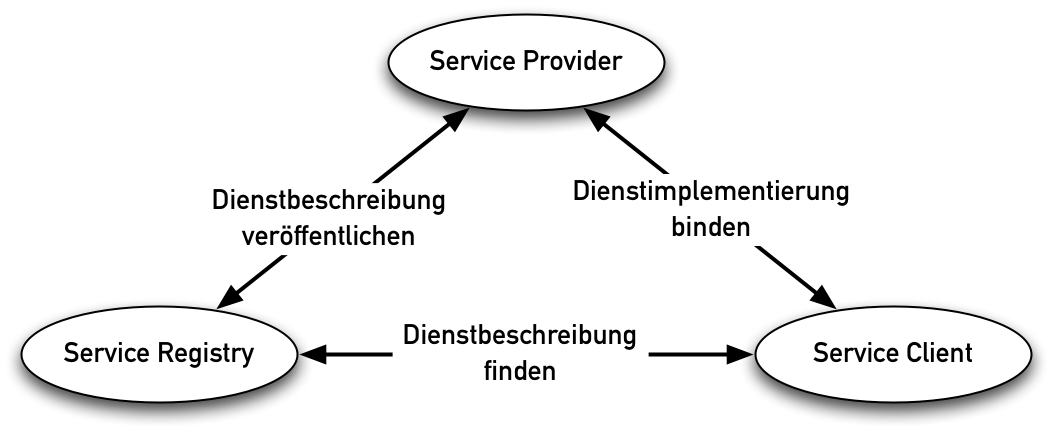
\includegraphics[width=.9\textwidth]{images/Basic_SOA.png}
  \caption{Einfachste Form einer dienstorientierten Architektur (nach~\citep{service_oriented_computing})}
  \label{fig:images_Basic_SOA}
\end{figure}

  In einer dienstorientierten Architektur wird aber voraus gesetzt, dass die einzelnen Dienste möglichst lose gekoppelt sind~\citep[S. 162]{soa_goes_real}. Um diese Kopplung zwischen den Dienste aufzubrechen, kann die Information welche Dienste miteinander interagieren sollen, in Form der \emph{Servicekomposition} externalisiert werden.

  Durch die Servicekomposition kreieren Entwickler Applikationen innerhalb von dienstorientierten Architekturen. Die Servicekomposition setzt dabei auf die grundlegenden Elemente einer SOA auf~\citep[S. 51]{milanovic2004csw} und stellt damit ein zentrales Element dar, um überhaupt aus einer Reihe von einzelnen Diensten eine Applikation zu aggregieren.
  
  Nach~\citep[S. 104]{masak2007ssb} kann die Servicekomposition dabei aus zwei unterschiedlichen Perspektiven betrachtet werden: der \emph{Geschäftsprozesskomposition} und der \emph{Servicelevelkomposition}. Bei der Geschäftsprozesskomposition werden "`völlig neue Geschäftsprozesse aus bestehenden Teilprozessen oder Services"' (\citep[S. 104]{masak2007ssb}) komponiert. Eine Einbettung in eine Organisation steht hier klar im Vordergrund. Bei der Servicelevelkomposition steht vielmehr "`die Interoperabilität und technische Machbarkeit im Vordergrund"' (\citep[S. 105]{masak2007ssb}) und es wird keine Rücksicht auf eine mögliche Organisationstruktur genommen. Da eines der Ziele von COSIMA die Entwicklung von Multimedia-Applikationen ist (vgl. Abschnitt \ref{sec:ziele_cosima}) und nicht die Abbildung von Geschäftsprozessen im Vordergrund steht, wird dieser Aspekt in dieser Arbeit nicht weiter verfolgt.
  
\subsubsection{Kompositionsarten} % (fold)
\label{ssub:kompositionsarten}

  Bei der Komposition von Diensten werden in der Literatur unterschiedliche Arten unterschieden. Die beiden grundsätzlichen, für COSIMA relevanten, werden bei Papazoglou in~\citep[S. 41]{papazoglou2007soc} genannt: \emph{Orchestrierung} und \emph{Choreographie}. Im Folgenden sollen diese beiden Ansätze genauer betrachtet werden.
  
\paragraph{Orchestrierung} % (fold)
\label{par:orchestrierung}
  
  Orchestrierung wird von Papazoglou wie folgt definiert:
  
  \begin{quote}
    \emph{"`Orchestration describes how services interact at the message level, including the business logic and execution order of interactions under control of a single end point. It is an executable business process that can result in a long-lived, transactional, multistep process model."'} (\citep[S. 41]{papazoglou2007soc})
  \end{quote}
  
  Wesentlich sind also die Interaktionen verschiedener Dienste, die von einer zentralen Stelle über einen Nachrichtenaustausch koordiniert und kontrolliert werden. Des Weiteren ist das Ergebnis ein ausführbarer Geschäftsprozess.

% paragraph orchestrierung (end)

\paragraph{Choreographie} % (fold)
\label{par:choreographie}

  In der Definition von~\citep{peltz2003wso} wird der Unterschied zwischen Choreographie und Orchestrierung deutlich:
  
  \begin{quote}
    \emph{"`[...] choreography, which is more collaborative and allows each involved party to describe its part in the interaction. Choreography tracks the message sequences among multiple parties and sources --- typically the public message exchanges that occur between Web services --- rather than a specific business process that a single party executes."'} (\citep[S. 46]{peltz2003wso})
  \end{quote}

  Choreographie verfolgt also einen dezentralen Ansatz; Es gibt nicht eine Instanz, die den Nachrichtenfluss kontrolliert, vielmehr tritt der Nachrichtenfluss zwischen den einzelnen Diensten in den Vordergrund.
  
  Bei der Betrachtung beider Ansätze wird deutlich, dass die Trennung von Choreographie und Orchestrierung eher künstlich erscheint und man stimmt bereits darüber überein, dass sie beide in einer Sprache und Umgebung\footnote{Zur Umsetzung dieser beiden Kompositionsansätze existieren zahlreiche, unterschiedliche Technologien und (Sprach-)Standards, deren weitere Betrachtung nicht mehr Teil dieser Arbeit sein kann.} vereint werden sollten~\citep[S. 42]{papazoglou2007soc}.

% paragraph choreographie (end)

% subsubsection kompositionsarten (end)

\subsubsection{Relevanz fuer COSIMA} % (fold)
\label{ssub:relevanz_fuer_cosima_komposition}

  Es wurde deutlich, dass die Servicekomposition für eine dienstorientierte Architektur von elementarer Bedeutung ist. Jedoch wurde auch klar, dass die Servicekomposition in COSIMA noch nicht so verstanden wird, wie sie in der Literatur verstanden wird; Dort findet eine Betrachtung im Kontext von Geschäftsprozessen statt. Sowohl in der bisherigen Zieldefinition von COSIMA, als auch in dem Szenario für die prototypische Realisierung der Architektur, dass in Kapitel~\ref{cha:szenario} vorgestellt wird, liegt der Fokus jedoch nicht auf Geschäftsprozessen. Daher ist auch eine weitere Betrachtung der genannten Details für diese Arbeit nicht notwendig. Dennoch kann festgehalten werden, dass es sich am ehesten um eine Orchestrierung handelt: Es existiert eine zentrale Komponente über die der Anwendungsentwickler die Möglichkeit erhält, die unterschiedlichen Funktionalitäten der Multimedia-Applikationen zu komponieren und in eine definierte Abfolge zu bringen.
  
  Aus den hier genannten Gründen kann auch bei der prototypische Realisierung auf die Verwendung einer existierenden Prozessbeschreibungssprache verzichtet werden.

% subsubsection relevanz_fuer_cosima (end)

  % - Definitionen von "`Workflow"' und "`Prozess"' in Zusammenhang auf die Entwürfe (vielleicht )
  % - BPEL/Orchestrierung/Choreographie mit Quellenangaben erläutern
  % - vielleicht macht dieser Abschnitt überhaupt keinen Sinn!
  % - Die grundsätzliche Möglichkeit der Verwendung einer Prozessbeschreibungssprache diskutieren
  
% subsection service_komposition (end)

\subsection{Infrastruktur und ESB} % (fold)
\label{sub:infrastruktur}

  Innerhalb einer dienstorientierten Architektur besteht der Bedarf nach einer Infrastruktur, die in der Lage ist, die einzelnen Dienste zu verwalten und zu integrieren~\citep[S. 270]{web_services_principles_and_technology}. Neben der bereits separat vorgestellten Servicekomposition gehören auch die in diesem Abschnitt vorgestellten Elemente dieser, in der Literatur als \emph{Enterprise Service Bus} (ESB\abk{ESB}{Enterprise Service Bus}) bezeichneten Infrastruktur an.
  
  In~\citep{web_services_principles_and_technology} wird der Enterprise Service Bus wie folgt defniert:
  
  \begin{quote}
    \label{def:enterprise_serivce_bus}
    \emph{"`The Enterprise Service Bus is an open standards-based message backbone designed to enable the implementation, deployment, and management of SOA-based solutions with a focus on assembling, deploying, and managing distributed service-oriented architectures."'} (\citep[S. 270]{web_services_principles_and_technology})
  \end{quote}
  
  Nach dieser Definition wird durch den Einsatz eines ESB überhaupt erst die Realisierung und der Betrieb einer dienstorientierten Architektur ermöglicht. Darüber hinaus lässt sich festhalten, dass auch das "`Assembling"' der einzelnen Teile innerhalb der Architektur in den Aufgabenbereich des ESB fallen. Demnach kann die Servicekomposition in einer SOA auch als eine Teilmenge des ESB angesehen werden~\citep[S. 3]{enterprise_service_bus}.

  Neben der Servicekomposition werden von dem ESB noch eine Vielzahl weiterer Aufgaben übernommen, die jeweils die Punkte Implementierung, Deployment\footnote{Für das englische Wort "`Deployment"' kann in diesem Kontext keine adäquate deutsche Entsprechung gefunden werden. Aus diesem Grund wird "`Deployment"' sinngemäß nach der Beschreibung in der Wikipedia verwendet: \emph{"`Software deployment is all of the activities that make a software system available for use."'} (aus Wikipedia: \url{http://en.wikipedia.org/wiki/Software_deployment}, zuletzt abgerufen am 22.10.2008)} und Management unterstützen sollen. Die Aufgaben, die im ESB dabei mindestens implementiert sein müssen, sind in der folgenden Liste nach~\citep[S. 137]{soa_goes_real} und~\citep[S. 146]{masak2007ssb} dargestellt:
  
  \begin{itemize}
    \item Routing von Nachrichten
    \item Kommunikationsbus als Integrationsgrundlage
    \item Datentransformation und -zuordnung
    \item Prozess- und Regelausführung
    \item Überwachung der einzelnen Komponenten
    \item Adaptoren für Applikationen
    \item Bereitstellen von standardisierten Schnittstellen
  \end{itemize}

  Historisch gesehen ist ein ESB die Weiterentwicklung von EAI Brokern~\abk{EAI}{Enterprise Application Integration}, die bereits ähnliche oder die gleichen Funktionalitäten bereitstellen können~\citep[S. 146]{masak2007ssb}. Der Enterprise Service Bus verzichtet dabei aber auf den zentralistischen Integrationsansatz von EAI Brokern und etabliert anseinerstatt eine verteilte Integration~\citep[S. 4]{enterprise_service_bus}. Die einzelnen Funktionalitäten werden, um diese Verteiltheit zu erreichen, selbst wieder als Dienste realisiert ~\citep{enterprise_service_bus,masak2007ssb,papazoglou2007soc}. Durch die Aufteilung in einzelne Dienste und deren Verteilung innerhalb des Service Bus, kann dann auch von einer virtuellen Infrastruktur gesprochen werden~\citep[S. 136]{soa_goes_real}.
  
  Das COSIMA Projekt sieht bis zu diesem Zeitpunkt nur einen sehr rudimentären ESB vor\footnote{Gemessen an dem Umfang, wie er in der Literatur beschrieben wird und in kommerziellen Systemen vorkommt.}. Dennoch übernimmt auch der Enterprise Service Bus in COSIMA die gleichen Verantwortlichkeiten, einige davon sind jedoch für den Einsatz in Multimediaanwendungen adaptiert worden. Im Folgenden werden die für das COSIMA Projekt relevanten Komponenten des ESBs näher beschrieben.
  
\subsubsection{Nachrichtensystem} % (fold)
\label{ssub:nachrichtensystem}
  
  Im vorangegangen Kapitel wurde als eine Aufgabe des Enterprise Service Bus, die Vermittlung und Übertragung von Nachrichten zwischen den einzelnen Teilnehmern genannt. Das \emph{Messaging}, also die Nachrichtenvermittlung ist immer das Herzstück eines ESB~\citep[S. 77]{enterprise_service_bus} und daher auch in COSIMA. Die Nachrichtenvermittlung dient dabei dazu eine sehr schnelle, asynchrone und verlässliche Kommunikation zwischen Applikationen zu realisieren. Eine Nachricht selbst ist dabei ein wohl-definiertes, datengetriebenes Textformat~\citep[S. 60f]{web_services_principles_and_technology}.
  
  In COSIMA wurde sich für ein Nachrichtensystem nach dem \emph{Publish/Subscribe}-Pattern entschieden~\citep[S. 106]{enterprise_integration_patterns}. Es ist eine von vielen Formen, um asynchrone und verlässliche Kommunikation zu realisieren, die dabei etwas besser skaliert als andere Lösungen~\citep[S. 69]{web_services_principles_and_technology}. Zusammengefasst lässt sich die Funktionsweise dieser Form der Nachrichtenvermittlung wie folgt beschreiben:
  
  \begin{itemize}
    \item Ein \emph{Publisher} veröffentlicht eine Nachricht zu einem bestimmten Thema.
    \item Alle \emph{Subscriber}, die dieses Thema abonniert haben, erhalten genau eine Kopie dieser Nachricht.
  \end{itemize}
  
  Bei~\citep[S. 127]{soa_goes_real} wird darüber hinaus gesagt, dass es sich bei dieser Form der Nachrichtenvermittlung, um eine nicht-gerichtete Kommunikation handelt.
  
  In COSIMA selbst werden über das Nachrichtensystem vor allem Kontroll- und Synchronisationsdaten vermittelt. Die Kontrolldaten werden dabei von der Komponente der Servicekomposition versendet, und beinhalten Informationen wo und wie die medienverarbeitenden Komponenten ihre Daten beziehen können. Das Nachrichtensystem soll nämlich nicht die Medien selbst vermitteln. Für diese Aufgabe wurde eine dedizierte Komponente eingeführt, die in Abschnitt~\ref{sub:integration_von_medien} näher beschrieben wird. Auf die Synchronisationsdaten wird in Abschnitt~\ref{ssub:synchronisation} näher eingegangen.
  
% subsubsection nachrichtensystem (end)

\subsubsection{Persistenz} % (fold)
\label{ssub:persistenz}

  Um Daten zu dauerhaft ablegen zu können, ist innerhalb von COSIMA ein weiterer Dienst vorgesehen worden, der \emph{Shared Persistence Service}. Allerdings kann nur eine \emph{Consumer}-Komponente über diesen Dienst ablegen lassen. Umgekehrt kann nur eine \emph{Producer}-Komponente Daten über diesen Dienst wieder einlesen. Eine \emph{Transformer}-Komponente, kann nach dem Quelle-Komponente-Senke Prinzip keinen Zugriff auf dauerhaft abgelegte Daten erhalten.
  
  Innerhalb von COSIMA ist dieser Dienst noch sehr rudimentär modelliert. In der Literatur zu SOA findet sich keine dedizierte Komponente, um Daten persistent zu speichern; Diese Funktionalität kann durch jeden beliebigen Dienst bereitgestellt werden. Für COSIMA war es jedoch wichtig, diese Funktionalität explizit zu modellieren~\citep{bericht}\footnote{Nach dem  ursprünglichen Ziel von COSIMA war es tatsächlich noch sinnvoll einen zentralen Dienst bereitzustellen, der die persistente Speicherung von Daten übernimmt. Durch die stärkere Ausrichtung auf SOA und die Umorientierung zu einer Architektur an Stelle eines Rahmenwerks, ist diese Entscheidung jedoch zu überdenken.}.
  
  Die Komponente zur persistenten Speicherung von Daten wird in dieser Arbeit nicht weiter behandelt werden.

% subsubsection persistenz (end)

\subsubsection{Synchronisation} % (fold)
\label{ssub:synchronisation}

  Die bisher vorgestellten Komponenten der Architektur innerhalb des COSIMA-Projekts sind weitestgehend übertragbar auf Komponenten in anderen dienstorientierten Architekturen. Zur Umsetzung von Multimediaanwendungen sind aber noch weitere, medienspezifische Komponenten erforderlich. Die Definition von einem Multimediasystem nach Steinmetz gibt hierzu einen ersten Hinweis:
  
  \begin{quote}
    \emph{"`Ein Multimediasystem ist durch die rechnergesteuerte, integrierte Erzeugung, Manipulation, Darstellung, Speicherung und Kommunikation von unabhängigen Informationen gekennzeichnet, die in mindestens einem kontinuierlichen (zeitabhängigen) und einem diskreten (zeitunabhängigen) Medium kodiert sind."'} (\citep[S. 13]{multimedia_technologie})
  \end{quote}
  
  Multimediasysteme oder -Anwendungen unterscheiden sich von Nicht-Multimediaanwendungen vor allem durch eine zeitliche Komponente~\citep[S. 14]{multimedia_technologie}: Zwischen den Informationen, die in unterschiedlichen Medien kodiert vorliegen kann und muss ein Bezug hergestellt werden können. Dieser Bezug wird als \emph{Synchronisation} bezeichnet. Eine Definition für Synchronisation, die auch für COSIMA Verwendung findet~\citep[S. 27]{bericht} ist:
  
  \begin{quote}
    \emph{"`Synchronization in the context of multimedia refers to the mechanisms used by processes (also specific to multimedia) to coordinate their ordering in the time domain."'} (\citep[S. 401]{steinmetz1990spm})
  \end{quote}
  
  Synchronisation spielt im Kontext von Multimediaanwendungen also eine entscheidende Rolle und muss demnach explizit und prominent modelliert werden. Ein erster Ansatz zur Integration von Synchronisation in das COSIMA-Projekt sieht dazu eine dedizierte Komponenten innerhalb der Servicekomposition vor. Da eine dienstorientierte Architektur ohnehin stark ereignisorientiert sein sollte, um ein Maximum an Flexibilität zu erhalten~\citep[S. 96]{masak2007ssb} wurde im ersten Schritt auch eine ereignisorientierte Integration der Funktionalität zur Synchronisation vorgesehen.
  
  Die gesamte Thematik der Synchronisation ist sehr komplex und eine Vielzahl von Aspekten muss betrachtet werden~\citep[S. 27ff]{bericht}. In dieser Arbeit soll das grundsätzliche Konzept der Architektur im COSIMA-Projekt validiert werden, daher kann keine genauere Betrachtung der Synchronisation stattfinden.

% subsubsection synchronisation (end)

\subsubsection{Time Engine} % (fold)
\label{ssub:time_engine}

  Im Zusammenhang mit der Synchronisation von unterschiedlichen Medien innerhalb von Multimediasystemen wurde bereits die Relevanz der Zeit-Domäne erwähnt. Bertino und Ferrari stellen werden noch deutlicher:

  \begin{quote}
    \emph{"`One of the inherent characteristics of multimedia data is of being heavily time-dependent in that they are usually related by temporal relations which have to be maintained during their playout."'} (\citep[S. 612]{bertino1998tsm})
  \end{quote}
  
  Zeit spielt im Umgang mit Medien also eine wesentliche Rolle. Unterschiedliche Medien haben aber zumeist unterschiedliche zeitliche Einheiten\footnote{Ein Video wird zum Beispiel mit Bilder pro Sekunde angegeben}. Dennoch muss eine Synchronisation zwischen diesen Medien möglich sein. In COSIMA soll die \emph{Time Engine} Komponente eine System-inhärente Zeit realisieren, über die die heterogenen zeitlichen Repräsentationen einzelner Medien umgerecht werden können. Auf diesem Wege soll dem Anwendungsentwickler eine einfache Möglichkeit gegeben werden, Synchronisation in seinen Anwendungen zu implementieren.

  Auch diese Komponente ist noch wenig spezifiziert und wird daher in dieser Arbeit nicht weiter behandelt.
  
  Im Folgenden Abschnitt wird die Integration von Medien, in Form des Medienobjekts und des Medien Brokers, in die Architektur vorgestellt. Obwohl diese Komponenten laut Abbildung~\ref{fig:Kontextsicht_Architektur_COSIMA} Teil des Enterprise Service Bus sind, werden sie auf Grund ihrer Relevanz gesondert davon betrachtet.

% subsubsection time_engine (end)

% subsection infrastruktur (end)

\subsection{Integration von Medien} % (fold)
\label{sub:integration_von_medien}

  Innerhalb einer Architektur für Multimediaanwendungen spielen vor allem die Medien selbst eine zentrale Rolle. Demnach war eine besondere Betrachtung dieser Daten notwendig, die dazu geführt hat, das die Mediendaten dediziert modelliert wurden~\citep{bericht}. Ergebnis dieser Modellierung sind das Medienobjekt und der Media Broker, die beide hier näher beschrieben werden sollen.
  
\subsubsection{Medienobjekt} % (fold)
\label{ssub:medienobjekt}

  Es wurde bereits in Abschnitt~\ref{ssub:nachrichtensystem} erläutert, dass in einer dienstorientierten Architektur der Datenfluss durch die Nachrichtenvermittlung realisiert wird. In~\citep[S. 27ff]{bericht} werden aber Eigenschaften von Mediendaten beschrieben, die sich nicht mit dem Verständnis von Daten bei "`klassischen"' dienstorientierten Architekturen decken. Aus diesen Unterschieden wurde die folgende Liste der Anforderungen an das Medienobjekt extrahiert~\citep{bericht}:
  
  \begin{description}
    \item[Erweiterbarkeit] Das COSIMA-Projekt soll Verwendung zur Entwicklung von Multimediaanwendungen in sehr vielen Domänen finden. Daher muss das Medienobjekt sich an diese Domänen leicht adaptieren lassen. Dies könnte durch eine abstrakte Darstellung der Eigenschaften von Medien erreicht werden.
    \item[Metadaten] Dort wo Medien verwendet werden, findet sich in den meisten Fällen auch eine Beschreibung dieser Medien. Diese Metadaten sind daher ebenso als \emph{first-class citizen} zu betrachten und inhärent im Medienobjekt verankert sein.
    \item[Streaming] Beim Umgang mit Medien, vor allem mit kontinuierlichen Medien spielen fast immer auch Datenströme, oder auch \emph{Streaming} eine wesentliche Rolle~\citep[S. 14ff]{multimedia_technologie}. Aus diesem Grund muss das Medienobjekt Streaming explizit vorsehen. Eng verbunden mit dem Streaming ist die \emph{Dienstgüte}~\citep{multimedia_technologie} und muss daher ebenfalls berücksichtigt werden.
    \item[Verteilung] In einer dienstorientierten und damit potentiell verteilten Architektur müssen auch die Medien verteilt zu prozessieren sein. Innerhalb des Medienobjektes müssen also dementsprechende Voraussetzungen geschaffen werden.
  \end{description}

\begin{figure}[ht]
  \centering
    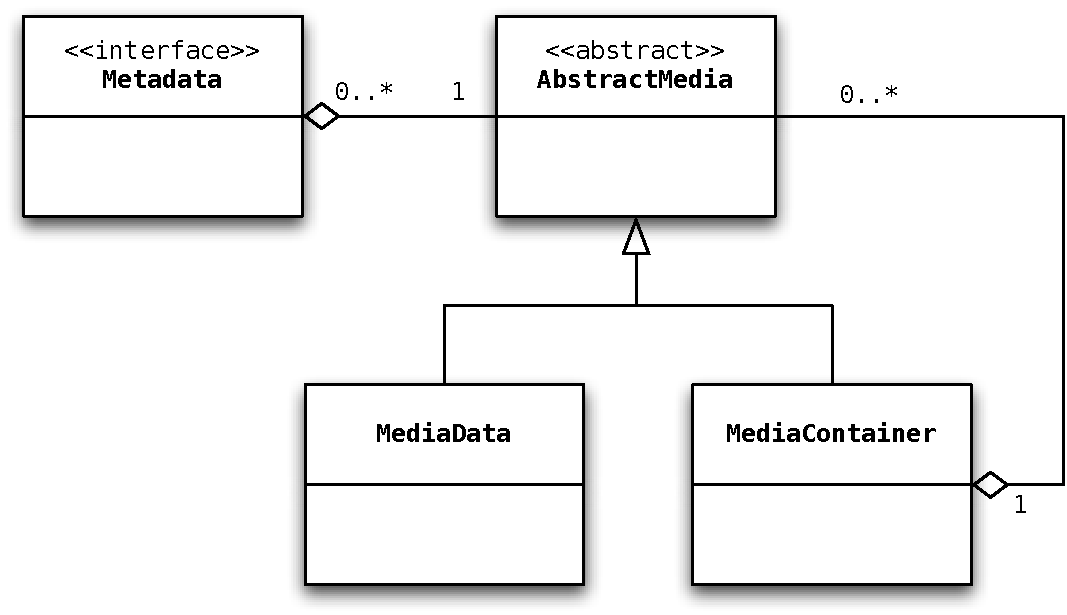
\includegraphics[width=.9\textwidth]{images/Medienobjekt.pdf}
  \caption{Vereinfachtes Klassendiagramm des Medienobjektes}
  \label{fig:medienobjekt}
\end{figure}

  Um diese Ziele zu erreichen, wurde das Medienobjekt nach dem \emph{Composite} Design Pattern entworfen~\citep[S. 163]{design_patterns}. Abbildung~\ref{fig:medienobjekt} zeigt das stark vereinfachte Klassendiagramm des Medienobjektes. Viele Punkte sind immer noch offen\footnote{So zum Beispiel ob die tatsächlichen Medien oder lediglich Referenzen auf Medien übertragen werden sollen.}, jedoch verspricht die jetzige Grundstruktur ein hohes Maß an Flexibilität bei der weiteren Umsetzung.
  
  Wie diese Medienobjekte innerhalb des Gesamtsystems vermittelt und übertragen werden sollen, stellt der folgende Abschnitt vor.

% subsubsection medienobjekt (end)

\subsubsection{Medien Broker} % (fold)
\label{ssub:media_broker}

  \begin{definition}[Broker]\label{def:broker}
    "`\textbf{1.} [engl. broker, eigtl. = Weinhändler]: Effektenhändler an der englischen und amerikanischen Börse."'\footnote{aus: Duden - Deutsches Universal Wörterbuch A-Z, 3. Aufl., 1996} "`\textbf{2.} One employed as a middleman to transact business or negotiate bargains between different merchants or individuals."'\footnote{aus: The Oxford English Dictionary, 3. Aufl., 1970} "`\textbf{3.} A middleman, intermediary, or agent generally; an interpreter, messanger, comissioner."'\footnote{aus: The Oxford English Dictionary, 3. Aufl., 1970}
  \end{definition}

  Als einen Broker kann man demnach einen Makler oder Vermittler zwischen zwei Parteien, die Informationen oder Waren austauschen wollen bezeichnen.

  Diese Bedeutung lässt sich auch im Umfeld von verteilten Systemen weitestgehend übernehmen\footnote{Hier ist beispielhaft der \emph{Object Request Broker} (ORB\abk{ORB}{Object Request Broker}) bei CORBA\abk{CORBA}{Common Object Request Broker Architecture} zu nennen~\citep{coulouris2001ds,balzert1999lo}.} und im Kontext der dienstorientierten Architekturen lässt sie sich auf den \emph{Message Broker} anwenden. Dieser stellt statt einer Punkt-zu-Punkt Verbindung zwischen Diensten, eine zentrale Vermittlungsstelle zur Verfügung~\citep[S. 71]{web_services}. Dabei muss es sich aber nicht immer um ein zentrales System handeln und wird in modernen Umgebungen zumeist als dezentrale Komponente realisiert~\citep{enterprise_service_bus}. Grundsätzlich kann auch gesagt werden, dass ein Broker dem \emph{Mediator} Pattern~\citep[S. 273]{design_patterns} in einer verteilten Umgebung entspricht~\citep[S. 83]{enterprise_integration_patterns}.
  
  Der Medien Broker bei COSIMA soll ähnliche Funktionen bei der Vermittlung von Medien zwischen den einzelnen Diensten übernehmen. Zur Zeit ist der Medien Broker so konzeptioniert, dass er die im vorherigen Abschnitt beschriebenen Medienobjekte zwischen den verschiedenen medienverarbeitenden Komponenten vermittelt.

% subsubsection media_broker (end)

% subsection medienobjekt (end)

% section architektur (end)

\section{Offene Fragen} % (fold)
\label{sec:offene_fragen}

  In diesem Kapitel ist der Status Quo des COSIMA-Projekts vorgestellt worden. Die bereits in~\citep{bericht} konzipierte Architektur wurde im Rahmen dieser Arbeit, vor allem bei der Verwendung der Begriffe aus der SOA-Domäne, weiter gefestigt. Das hier vorgestellte soll des Weiteren als Grundlage für die prototypische Realisierung und szenariobasierte Validierung dienen.

  COSIMA ist ein junges Projekt und daher gilt es noch viele Punkte zu klären. Im Folgenden sollen die wichtigsten dieser Punkte kurz erläutert werden. Nur wenige der Fragen, die dadurch aufgeworfen werden, können in dieser Arbeit beantwortet werden. Abschließend kann wohl auf keine einzige eine hinreichende Antwort gefunden werden.
  
\subsection{Framework oder Architektur} % (fold)
\label{sub:framework_oder_architektur}

  In der Zieldefinition und dem Mission Statement des Projekts, wie sie zu Beginn dieses Kapitels und in~\citep{bericht} genannt wurden, wird noch von der Erstellung eines \emph{Frameworks} gesprochen. Scherp und Boll nennen in~\citep[S. 396f]{scherp2006fe} die folgenden drei Punkte als Eigenschaften von Frameworks:
  
  \begin{itemize}
    \item Umkehrung des Kontrollflusses
    \item Vorgabe einer konkreten Anwendungsarchitektur
    \item Anpassbarkeit durch Variationspunkte
  \end{itemize}
  
  Ohne im Detail auf diese Eigenschaften einzugehen, fällt jedoch schnell auf, dass der Punkt zur Umkehrung des Kontrollflusses sich nur schlecht mit den Konzepten einer dienstorientierten Architektur decken lässt: Der Servicekomposition liegt nach~\citep[S. 320]{web_services_principles_and_technology} ein \emph{Flow-Model} zu Grunde, dass, wie bereits in Abschnitt~\ref{sub:service_komposition} detailliert beschrieben, den Ablauf einer Applikation steuert. Und diese unterliegt dem direkten Einfluss des Anwendungsentwicklers, wie in Abbildung~\ref{fig:Kontextsicht_Architektur_COSIMA} deutlich zu erkennen ist. Es ist demnach nicht mehr valide von einem \emph{Framework} zu reden, stattdessen sollte der Begriff \emph{Architektur} verwendet werden.

% subsection framework_oder_architektur (end)

\subsection{Servicekomposition} % (fold)
\label{sub:servicekomposition_fragen}

  Bei einer Weiterentwicklung muss in jedem Fall die Komponente der Servicekomposition weiter ausdifferenziert werden. Es muss eingehend die Eignung bestehender Sprachen zur Komposition von Diensten im Kontext von Multimediaanwendungen geprüft werden. Auch die Frage, ob eine Orchestrierung oder eine Choreographie vorzuziehen ist, oder eine Mischung aus beiden Ansätzen, wie sie auch bei~\citep{papazoglou2007soc} gefordert wird, muss geklärt werden.
  
  Ein weiterer Aspekt, der in den Verantwortungsbereich der Servicekomposition fällt, ist die Beachtung Nicht-Funktionalen Anforderungen einzelner Dienste~\citep[S. 42]{papazoglou2007soc}. Dieser Aspekt wurde bisher bewusst bei der Entwicklung des COSIMA-Projekts völlig ausgeblendet. Bei einer weiteren Entwicklung muss dieser Punkte daher unbedingt Berücksichtigung finden.

  Nach~\citep[S. 8]{service_oriented_computing} stehen im Kontext des \emph{Service-Oriented Computing} (SOC) komponierte Dienste für weitere Kompositionen zur Verfügung. Diese Möglichkeit ist zur Zeit nicht explizit in COSIMA modelliert worden. Auch für die Entwicklung von Multimediaanwendungen kann diese Fähigkeit von Vorteil sein. Welche Konsequenzen eine solche verschachtelte Komposition haben könnte, kann hier nicht abschließend geklärt werden und sollte daher Teil weiterer Forschung sein.

% subsection servicekomposition (end)

\subsection{ESB} % (fold)
\label{sub:esb_fragen}

  Bei der Realisierung eines Enterprise Service Bus muss die fundamentale Entscheidung getroffen werden, ob er API-getriebene oder Protokoll-getrieben implementiert werden soll~\citep[S. 59]{soa_in_practice}. Ohne diese beiden Ansätze an dieser Stelle weiter zu vertiefen, muss die Weiterentwicklung des Projekts sich für einen der beiden entscheiden.
  
  Es existieren eine Vielzahl von kommerziellen und nicht-kommerziellen ESB Lösungen. Deren Eignung für die Verwendung innerhalb des COSIMA-Projekts muss im Einzelnen geprüft werden, denn es ist deutlich geworden, dass die Entwicklung eines ESB komplex und aufwendig ist. Falls sie durch den Einsatz oder Anpassung einer bestehenden Implementierung minimiert werden kann, sollte entsprechend verfahren werden.

% subsection esb_fragen (end)

% section offene_fragen (end)

% chapter eine_dienstorientierten_multimediaarchitektur (end)
